\documentclass{acm_proc_article-sp}

%\usepackage{graphicx,fullpage,epsf,epsfig,endnotes}
\usepackage{graphicx}

\begin{document}

% remove the permissions block
\makeatletter
\let\@copyrightspace\relax
\makeatother

\title{Efficient Data-Intensive Computing and the Data Exchange Wall}
\numberofauthors{1}
\author{
\alignauthor
Tomer Shiran\\
       \affaddr{Carnegie Mellon University}\\
       \email{tshiran@cmu.edu}
\and
}
\date{15 April 2009}
\maketitle
\begin{abstract}
This paper describes a 12-week project that involves developing a model to help improve the performance and reduce the cost of data-intensive computing. This model will provide an in-depth understanding of the \emph{data exchange wall}, a phenomenon in which the overall throughput drops when a data-intensive program is executed on multiple machines. As CPUs become increasingly parallel (via multiple cores) and local storage bandwidth increases (via Flash or multiple disks per machine), the data exchange wall will become increasingly important and will need to be strongly considered in any data-intensive computing work. This project also involves extending DataSeries \cite{dataseries} to support parallel processing, both on a single machine (utilizing multiple CPUs and cores) and on multiple machines. Unlike other parallel dataflow systems, such as Hadoop \cite{hadoop}, Parallel DataSeries (PDS) will efficiently utilize local resources (disk and CPU), thus demonstrating the inefficiency of existing systems and allowing us to empirically corroborate our model.
\end{abstract}

\section{Background}
Large-scale parallel dataflow systems, such as MapReduce \cite{mapreduce} and Dryad \cite{dryad}, have attracted significant attention recently. They provide abstractions for specifying data-parallel computations, and they also provide environments for automating the execution of data-parallel programs on large clusters of commodity machines. MapReduce, in particular, has received a great deal of attention, and several implementations \cite{hadoop, phoenix} are publicly available. These programming models and systems offer an alternative to parallel databases \cite{paralleldatabases} for processing large data sets.


\section{Problem Statement}
In this section we identify two major problems that affect the data-intensive computing community.

First, there are no publicly available tools or models that help organizations and developers understand the bottlenecks of their parallel dataflow systems and applications. For example, developers do not know whether they should spend time optimizing the local (ie, per-machine) performance of their programs (eg, the map function in a map-reduce computation) or, instead, invest in reducing the amount of data exchange (ie, network traffic). Additionally, as a result of the data exchange wall, developers are sometimes better off running their computations on a single machine, even if they have access to multiple machines. However, developers currently do not have the tools to identify such cases. The lack of such tools also affects organizations that must decide how many machines to buy or rent. For example, there may be no benefit in buying a cluster of 10 machines over buying a single machine. Alternatively, it may be much less expensive to buy a single machine with more CPUs or disks than to buy a number of less-powerful machines.

Second, although existing systems can scale to hundreds and thousands of machines, they do not fully utilize the hardware resources on which they execute. For example, running Hadoop on a single machine and executing a grep-like program is more than an order of magnitude slower than running the standard UNIX grep command on the exact same hardware. As another example, Google's MapReduce implementation reaches a peak input data transfer rate of only 30 GB/s while running a distributed grep on a cluster of 1800 two-disk machines. That rate is equivalent to only 8.33 MB/s per disk at the peak, which is reached 60 seconds into the computation. This observation indicates that many individuals and organizations are spending excessive resources (capital and operating expenses) due to the inefficiency of existing parallel dataflow systems.

\section{Proposal}
This project will have several contributions. First, we will develop a simple model that will allow developers and organizations to understand the bottlenecks resulting from their specific combination of hardware, software and workloads. A developer that wants to run a data-intensive computation will use this model to reach design decisions, ranging from the target language (C++? Java?) to the choice of parallel algorithm. An organization that is planning to deploy a cluster for data-intensive computating will use this model to determine the ideal hardware configuration of the machines to purchase or rent. Figure \ref{fig:model} illustrates our initial model.

Second, we will show that existing systems, such as MapReduce and Hadoop, are highly inefficient, by analyzing publicly available results from those systems (eg, \cite{mapreduce}). The data exchange wall is masked by the inefficiency of such systems, because even for workloads with significant data exchange, the individual machines are unable to process enough data to saturate the network links.

Third, we will show that although existing systems, such as Dryad, have been shown to reach near-linear scalability on large clusters, such behavior has only been exhibited on workloads that are trivially parallel (ie, where data exchange between machines is negligible). The data exchange wall is masked by the lack of data exchange in such workloads, even if the system is highly efficient.

Fourth, we will develop Parallel DataSeries (PDS), a highly-efficient parallel dataflow system based on the open source DataSeries \cite{dataseries} system. PDS will significantly outperform existing systems, such as Hadoop, on several representative workloads (grep and sort). It will not only back our hypothesis that existing systems are inefficient, but also allow us to empirically corroborate our model by demonstrating scenarios that cannot be demonstrated with an inefficient system such as Hadoop.

Finally, we will propose directions for future research to address the inefficiency of parallel dataflow systems. For example, based on our model, we will discuss how disk/file and network compression could be utilized and tuned to improve overall throughput. 

\begin{figure*}[!b]
  \begin{center}
	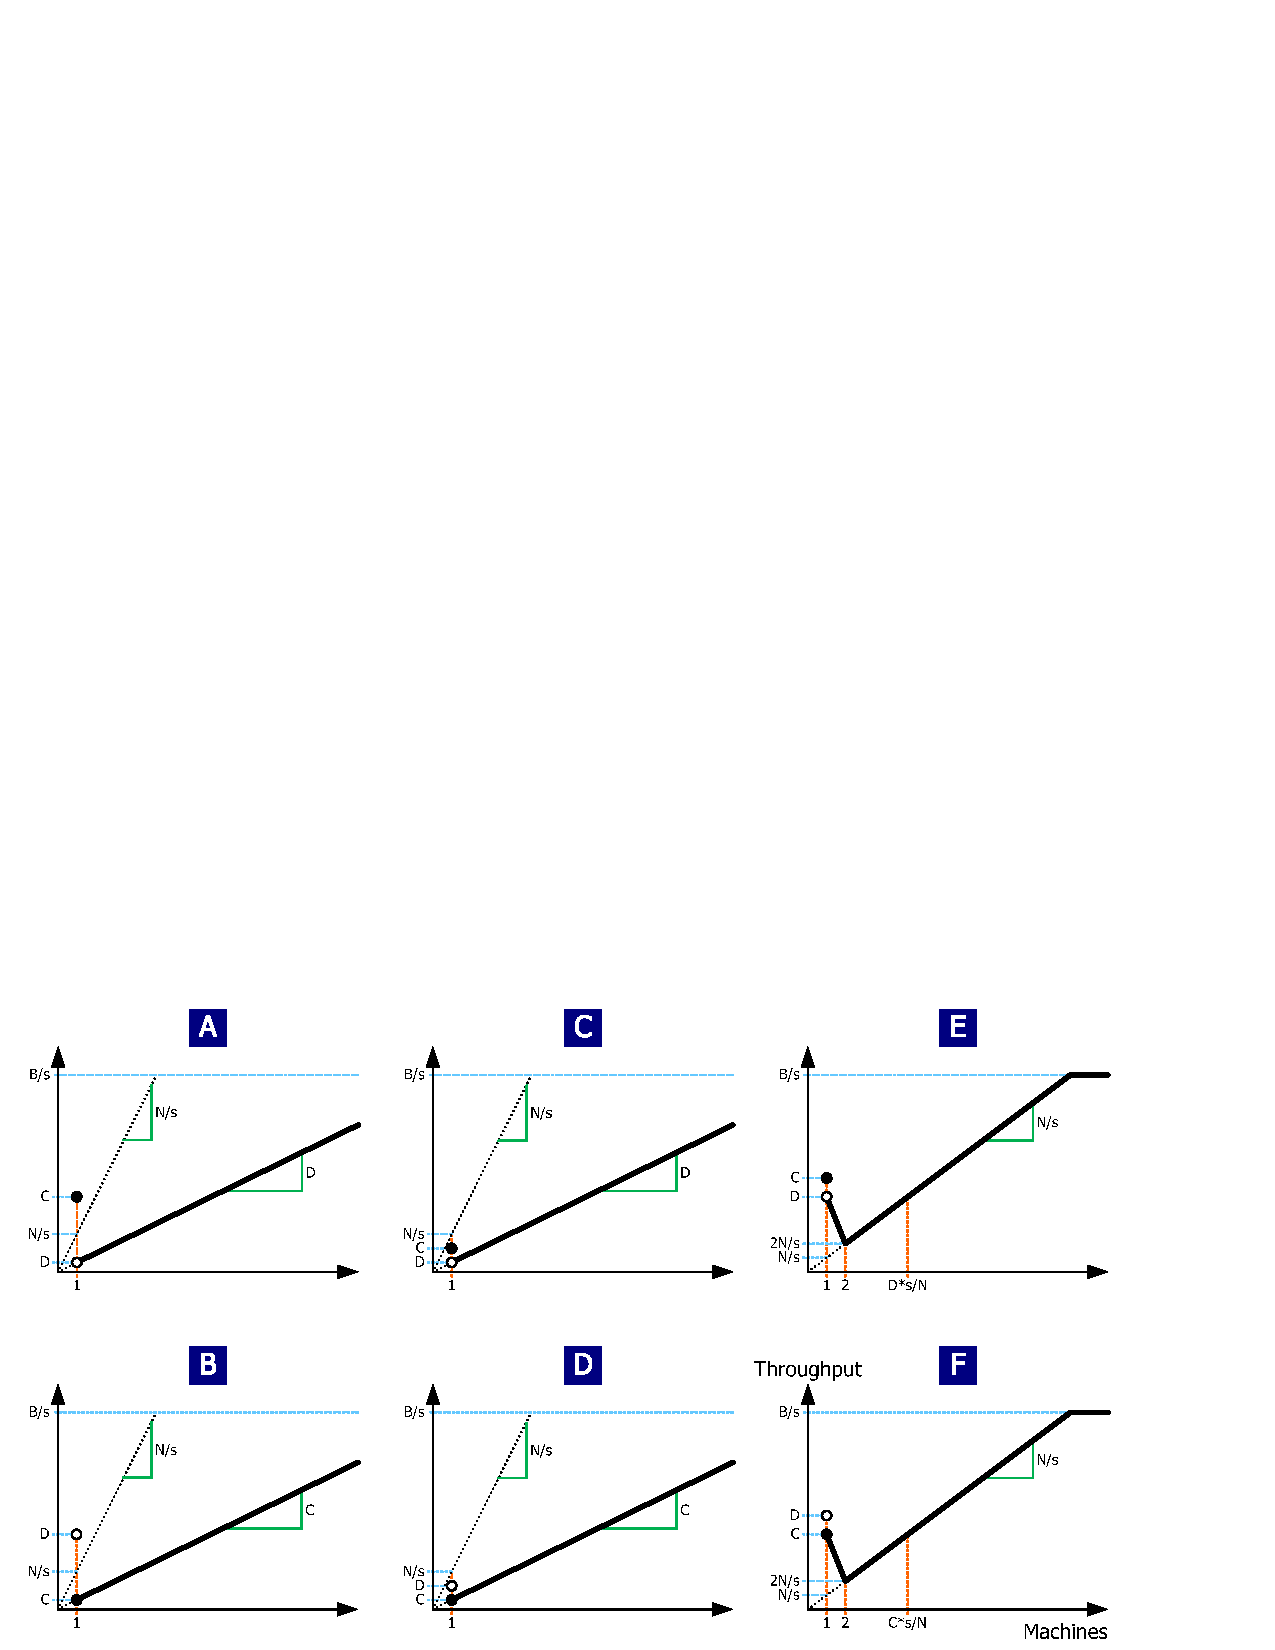
\epsfig{width=7in, angle=0, file=model} % model.vsd -> (Visio) model.pdf -> (pdf2ps) model.ps
  \end{center}

  \caption{\small The scaling properties of a data-intensive computation depend on the disk bandwidth (D), processing bandwidth (C) and network bandwidth (N) of the machines, the backplane bandwidth (aka bisection bandwidth, switch fabric) of the switch (B) and the ratio of input data that must be transmitted to other machines in the cluster (s) according to the parallel algorithm that is used. The relationship between the minimum of C and D (ie, the single-machine bottleneck) and N/s (the network bottleneck) is the most important factor, and also the one that determines whether the data exchange wall is present.}
  \label{fig:model}
\end{figure*}

\subsection{Parallel DataSeries}
A DataSeries program is organized as a pipeline of modules, in which the module that reads the data from a DataSeries file is a \emph{source}, and the module that writes the output data to a file is a \emph{sink}. All other modules in the pipeline are \emph{filters}.

PDS will allow developers to construct data-intensive programs that can efficiently utilize multiple CPU cores on a machine, and multiple machines in a cluster. Recalling that a DataSeries program is a pipeline of modules, achieving \emph{partitioned parallelism} \cite{paralleldatabases} is equivalent to allowing a module to run in parallel on multiple CPU cores and multiple machines.

PDS will use threading to achieve intra-process parallelism, and networking to achieve inter-process (ie, inter-machine) parallelism. Intra-process parallelism will enable PDS to achieve higher single-machine efficiency/throughput and will emphasize the significance of the data exchange wall in machines with multiple CPU cores. This is especially interesting in light of the overall industry trend towards CPUs with many cores.

\section{Experiments}
The purpose of developing PDS is to enable us to explore the different scenarios in our model -- primarily the difference between A-D and E-F (see Figure \ref{fig:model}). We will also run Hadoop and analyze why we do not experience the data exchange wall even with workloads that require significant data exchange (eg, sort). In order to reduce the effect of Hadoop's distributed file system (HDFS), we will try to run on an idle cluster to ensure maximum HDFS locality.

\subsection{Grep}
We will demonstrate scenarios A-D by implementing a distributed grep-like program that counts the number of occurrences of a given substring. We will vary the number of machines and plot throughput vs. number of machines (similar to Figure \ref{fig:model}). The graph will include two lines -- one for PDS and one for Hadoop. This experiment will demonstrate the impact of local efficiency (ie, the throughput of a single machine) on the throughput of data-intensive computations with minimal data exchange.

\subsection{Sort}
 We will demonstrate scenarios E-F by implementing a distributed sort program with partially-sorted input, ranging from random input to fully-sorted input, thereby varying the amount of data exchange (in the first phase of a distributed sort, each machine partitions its data and sends one partition to each machine, including itself, so the extent to which the data is already sorted determines how much data each machine will ``send'' to itself and how much it will have to send over the network). The graph will include multiple lines for PDS and one line for Hadoop (we will only test random input on Hadoop since we cannot control scheduling to the necessary extent). This experiment will demonstrate the impact of local efficiency as well as the amount of data exchange in a parallel algorithm on the throughput of data-intensive computations. A distributed sort execution with random data is expected to result in the most significant data exchange wall.

\section{Timeline}
The following table outlines the project's expected timeline.
\newenvironment{noop}{}{}
\begin{noop}\begin{tabular}{|c|c|p{2.2in}|} \hline
Week(s)&Date&Task\\ \hline
1 & 4/24 & Refine model and evaluate MapReduce and Dryad and according to model. Write corresponding sections of thesis/paper\\ \hline
2 & 5/1 & Write high-level design for PDS\\ \hline
3-4 & 5/15 & Implement intra-process parallelism (thread-based) in PDS\\ \hline
5-6 & 5/29 & Implement inter-process parallelism (RPC-based) in PDS\\ \hline
7-8 & 6/12 & Define dataflow graph specification format, and implement a system that reads the specification and runs the parallel program on the cluster\\ \hline
9-10 & 6/26 & Implement/run distributed grep experiment on PDS and Hadoop. Celebrate Reut's birthday!\\ \hline
11 & 7/3 & Implement/run distributed sort experiment on PDS and Hadoop\\ \hline
12 & 7/10 & Finish writing thesis/paper\\
\hline\end{tabular}\end{noop}

Although the project is currently scheduled to end on 7/10, we may need to stretch it in order to complete the proposed work (or at least enough to achieve interesting results). The hard deadline for the project is 8/14.

\section{Priorities and Non-Goals}
Due to the short time frame and limited resources, this project will focus only on achieving the specified goals. With regard to the design and implementation of PDS, the following functionality is important to a production system but is a not a goal for this project:
\begin{itemize}
\item Using or building a job scheduler. Instead, we will rely on ssh and simple scripts to manage the PDS processes on the cluster's machines.
\item Using or building a parallel filesystem, or automatically partitioning data sets. Instead, we will manually partition and distribute the desired data sets on the local filesystems of the machines.
\item Fault tolerance. Although large-scale systems are expected to deal with failures, we do not address such failures in this project.
\item Automatically determining an execution plan. Instead, we will require the user to specify the exact dataflow graph.
\item Automatically optimizing data packing and compression parameters for network transmissions. Instead, we will require the user to specify the desired settings in the specification of the dataflow graph.
\item Optimizing for power efficiency. Although power consumption is important, we will not specifically attempt to optimize it. However, by requiring less machines for a given task, our system will contribute to lower power consumption, and we may end up measuring the power savings.
\end{itemize}



%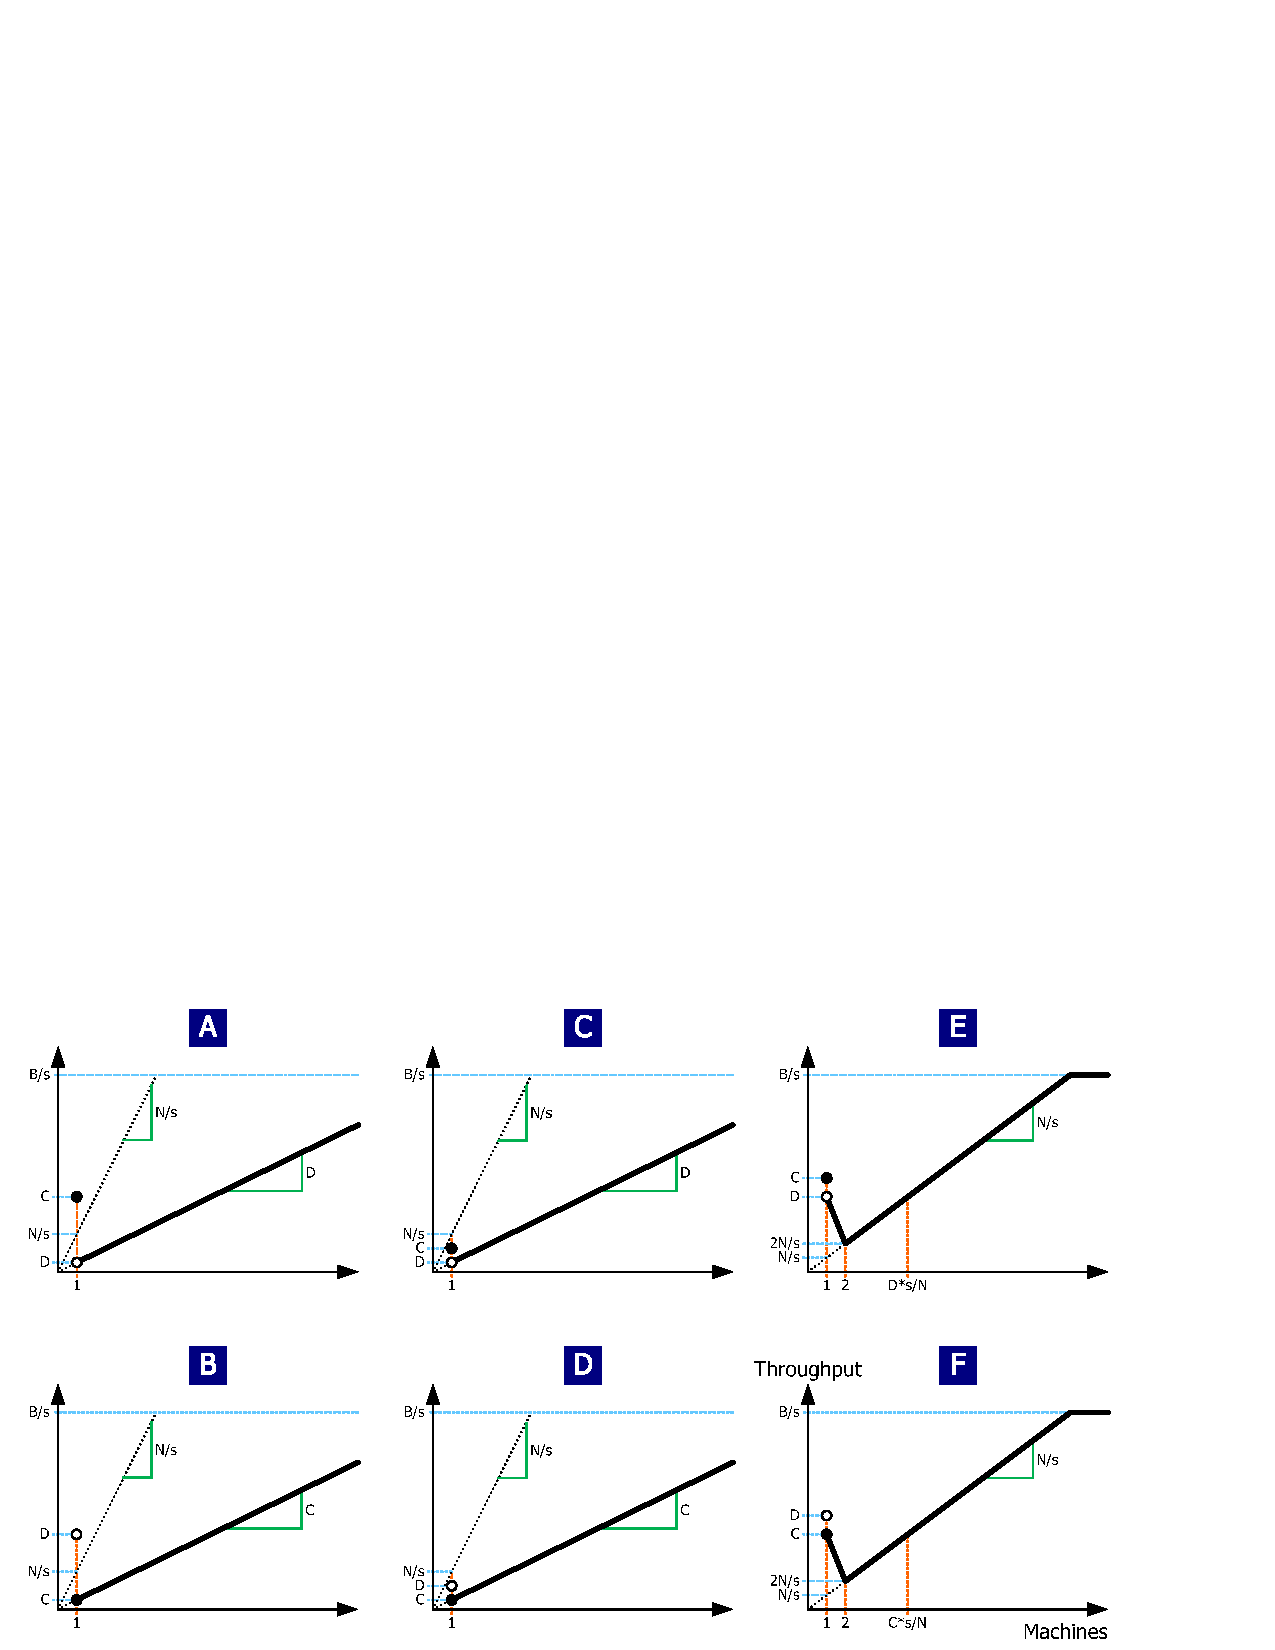
\includegraphics{model.png}

%\begin{figure*}[!b]
%  \begin{center}
%    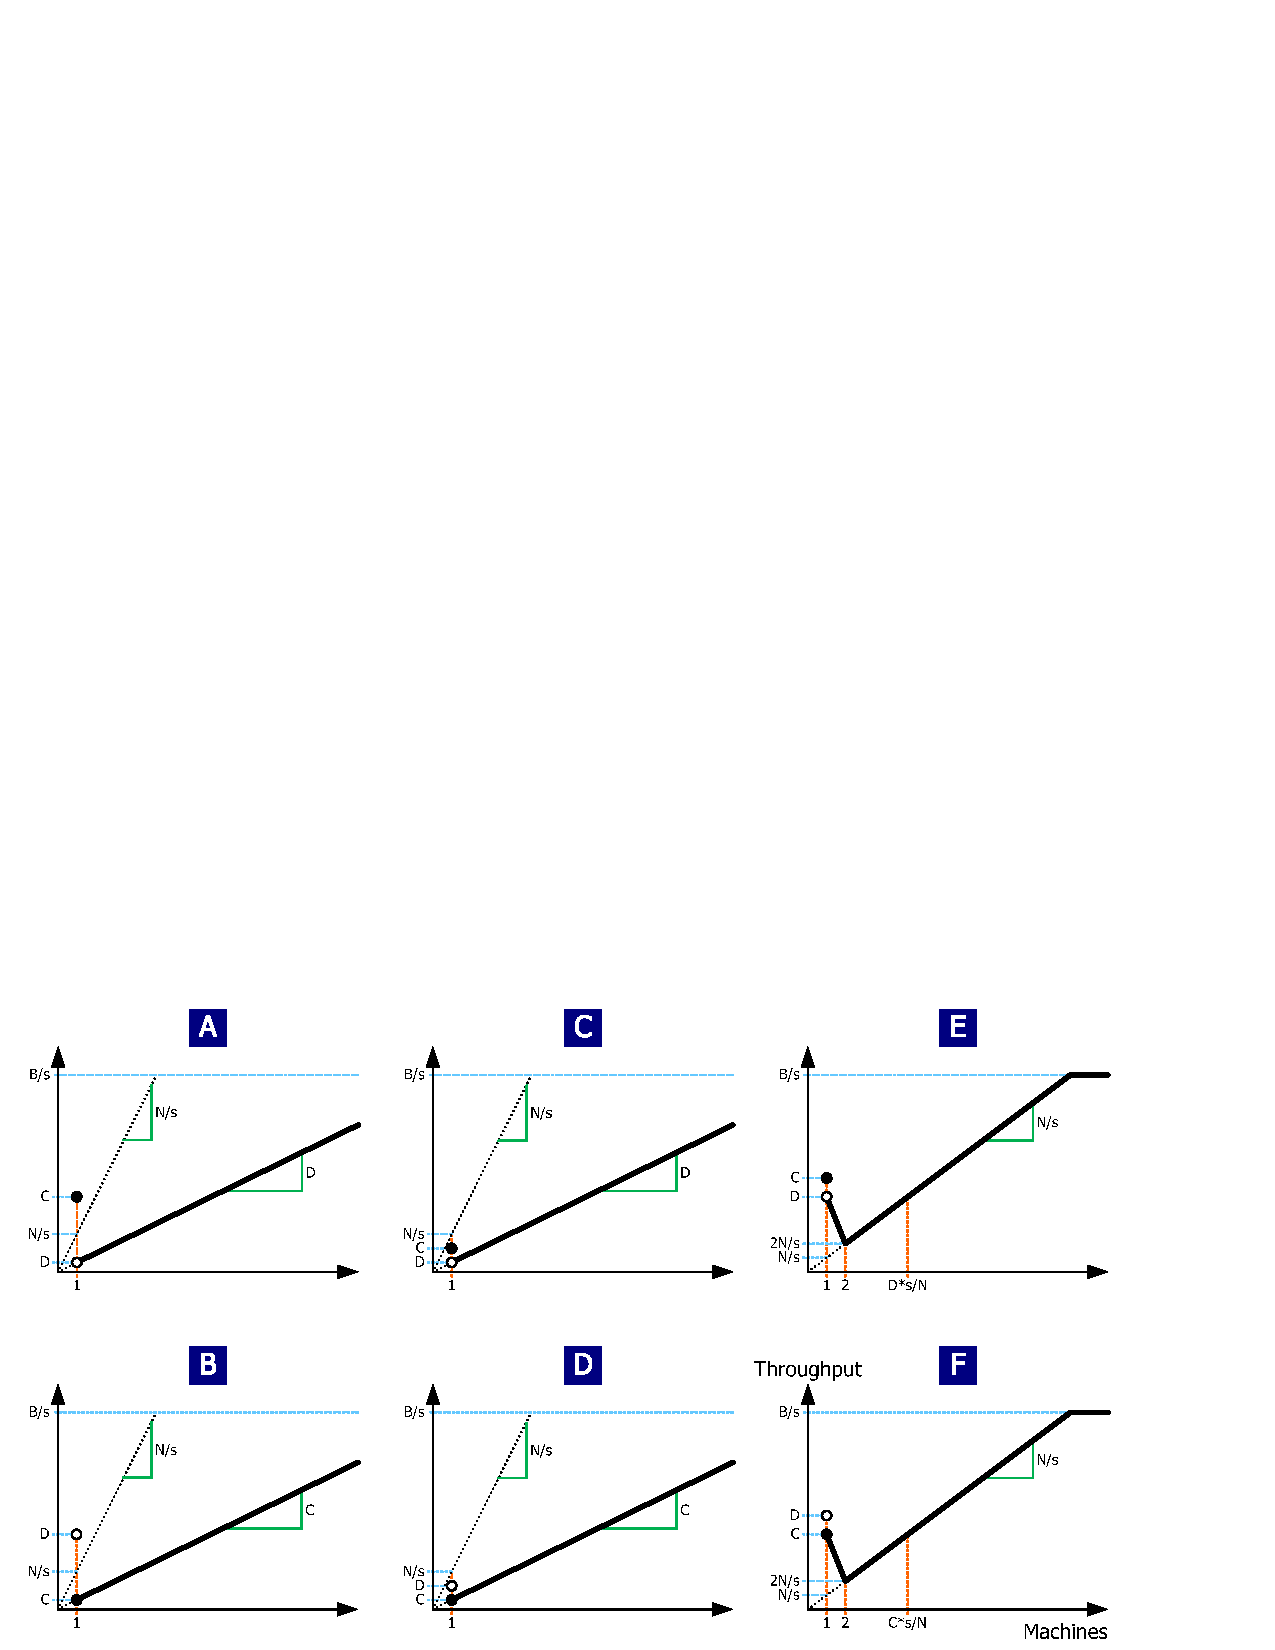
\includegraphics[width=3.5in]{model.png} % need to create PDF at home (Visio 2007)
%  \end{center}

%  \caption{\small Figure caption. To get a figure to span two
%      columns, use the environment figure* rather than figure.}
%  \label{model}
%\end{figure}

% NOTES FOR THE THESIS/PAPER
% What can we learn from the model?
% 1) The scalability slope cannot exceed N/s. Given sufficient disk and processing throughput, the slope will indeed be N/s (processing power depends on CPU(s), problem and implementation details).
% 2) The lowest throughput will be with either 1 or 2 machines. In the latter case, it will take min(C,D)*s/N machines to reach the throughput of a single machine, after which the increase will be at the N/s rate.
% 3) There are cases in which the lowest throughput is with 1 machine and the slope is N/s. This happens when N/s<min(C,D)<2N/s
% 4) We can play with C vs. D using disk/file compression. We can play with C/D vs. N/s using network compre

\section{Related Work}
Google's MapReduce \cite{mapreduce} offers a programming model that enables easy development of scalable parallel applications to process a vast amount of data on large clusters of commodity machines. Through a simple interface with two functions, map and reduce, this model facilitates parallel implementation of many real-world tasks such as data processing and machine learning. Hadoop \cite{hadoop} is an open-source map-reduce implementation for large clusters that is very similar to \cite{mapreduce}. MapReduce and Hadoop, unlike PDS, are highly inefficient due to various design and implementation details (eg, exchanged data is always written to disk before it is sent over the network).

Phoenix \cite{phoenix} is a shared-memory implementation of the map-reduce model for multi-core and SMP machines that allows programmers to develop parallel applications without having to deal with threading and synchronization. Due to its use of shared memory rather than temporary files and TCP networking, Phoenix can  outperform MapReduce on a single machine. Phoenix, unlike PDS, is designed to run only on a single machine.

Dryad \cite{dryad}, like MapReduce, offers a programming model and an execution framework for writing parallel distributed programs. A Dryad programmer writes several sequential programs and connects them using one-way channels. The computation is structured as a directed graph (similarly to \cite{paralleldatabases}). Dryad is responsible for executing the user-specified graph on a cluster of commodity machines. Dryad also handles fault tolerance, scheduling and resource management. Dryad is not publicly available, and its performance has only been measured and published on workloads that involve very little data exchange.

Additional, higher-level languages have been introduced on top of MapReduce, Hadoop and Dryad. These models further simplify the task of developing and executing scalable parallel applications. Sawzall \cite{sawzall} is a high-level language for the MapReduce framework that includes various built-in aggregators. Pig Latin \cite{piglatin} is a high-level procedural language for the Hadoop framework, which can also be executed on other frameworks (by extending Pig, the compiler that translates Pig Latin programs into Hadoop programs). Pig Latin offers various operators, such as COGROUP, FOREACH and FILTER, and is similar to the declarative SQL language. DryadLINQ \cite{dryadlinq} generates Dryad computations from the LINQ Language-Integrated Query extensions to C\#. Programs written in Sawzall, Pig Latin and LINQ are all translated to lower-level representations that can run on parallel dataflow systems, and it would be easy to adapt them to support PDS.

Gordon \cite{gordon} is a system architecture for data-intensive applications that combines low-power processors, flash memory and parallel dataflow systems (eg, Hadoop) and improves the performance and power-consumption of such applications. Gordon focuses on identifying the best hardware for large-scale parallel processing. According to trace-based simulations (Gordon is not an actual system), Gordon can outperform disk-based clusters by 1.5x. However, the simulations do not account for networking, which is often the bottleneck in such applications. Furthermore, Gordon assumes a given software stack and, unlike PDS, does not address the relationship between the system's hardware and software.

\section{Week 1}
\subsection{Grep on MapReduce}
A distributed grep execution on MapReduce involved 1800 machines, each consisting of two 160 GB IDE disks and a gigabit Ethernet link. \cite{mapreduce} does not provide the specifications or model numbers of the disks. However, we can estimate the sustained throughput of such disks by looking at publicly available data. The specifications of a Barracuda 7200.10 Ultra ATA/100 160 GB drive indicate a sustained throughput of 78 MB/s \cite{seagate160gb}, so we assume that the disks measured in \cite{mapreduce} had similar throughput. In other words, any of the 1800 machines in the MapReduce cluster could read input data off its disks at a rate of $D = 2 \cdot 78 = 166 \text{ MB/s}$.

We cannot determine the value of $C$ because it is implementation-dependant. Also, since a selective grep operation hardly requires any data exchange (if at all), we assume that $s = 0$ and $N/s$ is undefined (ie, very large), indicating a workload that cannot be network-bound. According to our model, the system's expected aggregate throughput is $n \cdot min\{C, D, N/s\} = 1800 \cdot min\{C, 166 \text{ MB/s}\} = min\{1800C, 1800 \cdot 166 \text{ MB/s}\} = min\{1800C, 298800 \text{ MB/s}\}$. The experiments indicated that the system reached a peak throughput of 30000 MB/s and an average throughput of about 15000 MB/s (according to the provided graph). Considering the peak throughput, we have $C=30000/1800=16.67\text{ MB/s}$. 

Referring to our model, $C < D$. It is worth noting that MapReduce reads its input data from GFS \cite{gfs}, and in some cases input files may need to be transmitted over the network. However, this is unlikley to affect the relationship between $C$ and $D$ because:
\begin{itemize}
  \item The experiments were executed during the weekend on an idle cluster. Thus, MapReduce's locality optimization  ensured that most mappers were scheduled to run on the machines that actually stored their input files (this is explicitly mentioned in the paper's description of the sort experiment).
  \item Even if locality was not achieved on some machines, $D$ would only drop to about 100 MB/s on gigabit Ethernet, still much higher than $C$.
\end{itemize}

Judging the distributed grep experiment on MapReduce in light of our model emphasizes several points:
\begin{itemize}
  \item MapReduce only utilizes 10\% of the available disk throughput.
  \item For workloads with little data exchange (like grep), MapReduce would benefit most from a more efficient implementation (or faster CPUs).
\end{itemize}

\subsection{Sort on MapReduce}
Our analysis of the distributed sort experiment on MapReduce is similar to that of distributed grep, except that we must account for the data exchange. In a distributed sort with random input, the amount of data that is transmitted over the network (as part of the data exchange) is roughly the same as the amount of input data. Since $N = 100 \text{ MB/s}$ on gigabit Ethernet, we have $N/s = 100/1 = 100 \text{ MB/s}$. The aggregate input rate peaked at 13000 MB/s and the aggregate data exchange rate peaked at 5000 MB/s. Thus, we have $5000 = n \cdot min\{C, D, N/s\} = 1700 \cdot min\{C, 166 \text{ MB/s}, 100 \text{ MB/s}\}$. Therefore, $C = 5000/1700 = 2.94 \text{ MB/s}$.

As in grep, the throughput of distributed sort on MapReduce is severely limited by the system's processing overhead. Given that the map phase of sort only involves partitioning the data, we would expect an efficient system to be I/O-bound (in this case, $N/s < D$, so we would expect it to be network-bound). Given that the network had about 100-200 Gbps at the root, we can conclude that the maximum aggregate throughput is $B/s = 10000/1 = 10000 MB/s$ (assuming, very conservatively, that the root had 100 Gbps and that all data exchange crossed the root switch). With an efficient system, this would be reached with only $(B/s) / (N/s) = 10000/100 = 100$ machines. In other words, an efficient system would reach twice the aggregate throughput of MapReduce with 17 times less machines. We further suspect that a higher backplane bandwidth ($B$) would be possible (with 100-200 machines, as opposed to 17000), thereby allowing the efficient system to scale beyond 100 machines and 10000 MB/s.

\subsection{Data Mining on Dryad}
\cite{dryad} describes an experiment involving a cluster of 1800 machines with four disks and one gigabit Ethernet link. The exact model of the disks is provided. Their sustained transfer rate, according to \cite{wd400gb}, is 65 MB/s. Given that the input data was striped across all four disks, the aggregate disk throughput (for sequential reading) on a single machine is $D = 4 \cdot 65 = 260 \text{ MB/s}$.

The end-to-end computation of this experiment took 11.5 minutes, processing a total of 10160519 MB, so the aggregate input throughput was $T = 10160519 / (11.5 \cdot 60) = 14725 \text{ MB/s}$. The workload performed a significant data reduction; of the 10160519 MB of input data, only 153703 MB were transmitted in the first data exchange, so we have $s = 153703 / 10160519 = 0.015$ and $N/s = 100/0.015 = 6667 \text{ MB/s}$ (assuming a throughput of 100 MB/s for gigabit Ethernet). According to our model, we have $14725 = n \cdot min\{C, D, N/s\} = n \cdot min\{C, 260 \text{ MB/s}, 6667 \text{ MB/s}\}$. We can clearly see that both the disks and the individual network links do not limit the throughput. Furthermore, given that the cluster was of similar size to the one in the MapReduce experiments, we will assume that $B = 10000 \text{ MB/s}$. We then have $B/s = 10000/0.015 = 666667 \text{ MB/s}$, so clearly the network's backplane bandwidth is not the limiting factor either. We must therefore conclude that $C = 14725 / 1800 = 8.18 \text{ MB/s}$, over 30 times slower than the available disk throughput. The performance of Dryad is severely limited by the processing throughput of the individual machines. Since the machines have sufficient CPU and memory to read at the maximum input rate supported by the disks (the second-slowest link in the chain), we conclude that the system's implementation is inefficient. Even if we assume that 10\% of the overall time was spent on startup, and that only 75\% of the execution time was spent in the first phase (the Q' vertices in Figure 10 of \cite{dryad}), we have $T = 21814.81 \text{MB/s}$ and $C = 14725 / 1800 = 12.12 \text{ MB/s}$, still over 20 times less than the available disk throughput. The assumption that over 75\% of the actual execution time was spent on the first phase is reasonable because the first phase reduces the amount of data by a factor of $1/s = 66$, and none of the remaining phases  (two layers of a merge sort followed by a count) should take a significant amount of time.

\bibliographystyle{abbrv}
\bibliography{pds}

\balancecolumns
\end{document}
